\documentclass{article}
\usepackage{float}
\usepackage{graphicx}
\author{Simone Abelli, Stefano Azzone}
\title{DIMA Project report: MBox}
\begin{document}
\maketitle
\newpage
\tableofcontents
\newpage
\section{Introduction}
\subsection{Purpose}
The purpose of this document is to provide more technical and detailed
information about the mobile application developed. The Design Document is a
guide for the programmer that will manage the future development of the codebase
for the application in all its functions. The document will explain and motivate
all the architectural choices by providing a description of the components and
their interaction. We will also enforce the quality of the product through a set
of design characteristics. Finally we describe the implementation, integration
and test planning.
The topics touched by this document are:
\begin{itemize}
	\item high level architecture
	\item main components, screens and widgets
	\item runtime behavior
	\item design patterns
	\item more details on user interface
	\item requirements and their mapping on the architecture
	\item implementation and test planning
\end{itemize}

\subsection{Scope}
MBox is an application for mobile devices that allows users to access all the
music present on their devices without having to worry about manually managing 
the metadata. The target user has basic knowledge of the functions of the
mobile device (e.g. is able to interact with the filesystem). Since the
application is focused on users who want to listen to music, which is usually
done with a portable device, we will focus smartphones maily (the application
also works on tablets). For the development of this applications we have decided
to use flutter since it's a framework thought for multiplatform deployment.

\subsection{Glossary}
\paragraph{Queue:} a queue is a data structure containing a list of tracks
which are to be played according to a FIFO policy.
\paragraph{Metadata: } metadata are information of a track regarding the track
itself (e.g. track title, artist, album cover \ldots)

\newpage

\section{Description and requirements}
\subsection{Product description}
MBox has all the functionalities of a music player:
\begin{itemize}
    \item Detect music present in the Music folder
    \item Allow management of playlists
    \item Organize music by artist, album and playlist
    \item Allow to arrange tracks in a playback queue
    \item Play tracks (in random order if desired)
    \item Visualize metadata related to tracks
\end{itemize}
In addition to this, MBox allows a more advanced and automated metadata
management, and the access to other music information:
\begin{itemize}
    \item Automatically set missing metadata (Title, Artist, Album, Cover,
        Lyrics, Track number, Artist image, \ldots)
    \item Manually edit metadata
    \item Visualize information about artists like a brief description, albums
        and other songs
    \item Search on the internet for other songs and listen to them
\end{itemize}

\subsection{Assumptions}
\begin{itemize}
    \item When downloading metadata or looking for other music, internet
        connection is available
    \item The user is able to move their music to the Music folder
    \item The tracks are present on Spotify to download metadata
    \item When the user looks for a track not present on their device, it must
        be present on YouTube
    \item The tracks are in mp3 format (otherwise metadata management is harder)
    \item The access to the filesystem is granted
    \item The device on which the application is used has some means to 
        play music
\end{itemize}

\subsection{Functional requirements}
\begin{enumerate}
    \item The application can access the filesystem and fetch songs from the
        music folder
    \item The application can play the selected tracks
    \item The application allows the user to add or remove tracks from the
        playback queue
    \item The application allows the user to pause and resume playback
    \item The application allows the user to skip tracks in the queue
    \item The application should save the queue state to resume playback if the
        application is closed
    \item The application allows the user to add or remove playlists
    \item The application allows the user to add or remove tracks from playlists
    \item The application organizes the tracks by artist and album
    \item The application allows the user to view lyrics of currently playing 
        track
    \item The application allows the user to edit metadata of the tracks
    \item The application automatically adds missing metadata using an external
        service (in our case Spotify); already present metadata is kept
    \item The application can show information about the artists of the tracks
        present on the device (such as all their albums and tracks)
    \item The application allows the user to search for tracks not present on
        their device, and play them through an external service (in our case
        YouTube)
    \item It should be possible to use the application without an internet
        connection, obviously with limited functionalities (no external song
        search, metadata editing \ldots)
\end{enumerate}

\subsection{Non functional requirements}
\begin{enumerate}
    \item The application should feel snappy and responsive
    \item The application layout should be intuitive to use
    \item The application should be reliable
\end{enumerate}
\newpage

\section{Architectural Design}
\subsection{Architectural Style and Patterns}
The application is logically subdivided in a frontend and a backend.
The frontend presents the information to the user and allows them to interact
with the backend. The backend contains and manages all the data and interfaces
with the external services.
\subsubsection{Frontend}

\begin{figure}[H]
	\noindent
	\makebox[\textwidth]{ 
		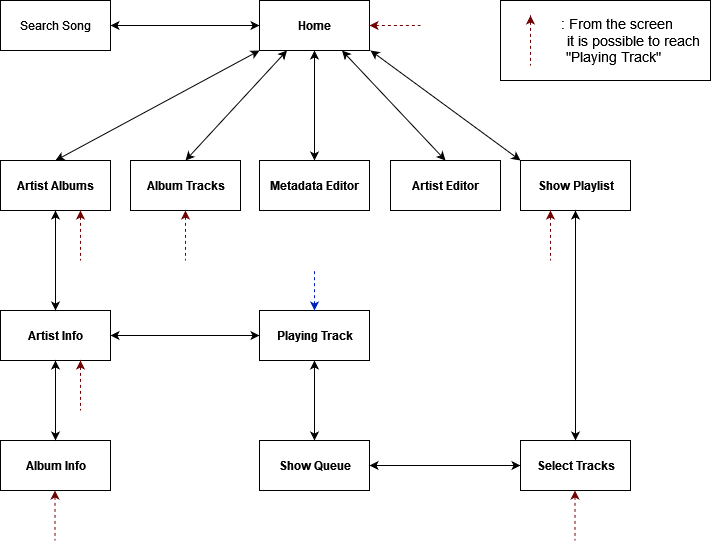
\includegraphics[scale=0.6]{images/ScreensDiagram.png}}
	\caption{Frontend system architecture} 
\end{figure}

The frontend is composed by the screens of the application. Once opened MBox
shows the \textbf{Home} screen. The Home screen is composed by 4 tabs:
\begin{itemize}
    \item \textit{Tracks}: a list of the tracks in alphabetical order; by
        selecting one we switch to the \textbf{PlayingTrack} screen, and start
        playing that track.
    \item \textit{Albums}: a list of the albums in alphabetical order; by
        selecting one we switch to the \textbf{AlbumTracks} screen, where we can
        select a track to play. 
    \item \textit{Artists}: a list of the artists in alphabetical order; by
        selecting one we switch to the \textbf{AlbumArtists} screen, where  we
        can select an album to show.
    \item \textit{Playlists}: a list of the playlists in alphabetical order; by
        selecting one we switch to the \textbf{ShowPlaylist} screen, from which
        we can start the playback; in the Playlists tab it is also possible to
        add a new playlist or remove an existing one.
\end{itemize}

By keeping a track pressed it is possible to open a drop down menu with a few
entries:
\begin{itemize}
    \item \textit{Edit metadata}: switch to the \textbf{MetadataEditor} screen
        to modify the metadata of the track
    \item \textit{Add to queue}
    \item \textit{Add to playlist}
\end{itemize}

By keeping an artist pressed it is possible to switch to the
\textbf{ArtistEditor} screen in order to change its image.

By touching the magnifying glass in the top right corner of the application, it
is possible to reach the \textbf{SearchSong} screen that allows the user to look
for songs that are not present on their device, and play them through an
external service (in our case YouTube).
\\\\
From the \textbf{PlayingTrack} screen it is possible to:
\begin{itemize}
    \item \textit{pause} and \textit{resume} playback
    \item \textit{skip} forward and backward in the queue
    \item \textit{change playback position} of the currently playing track
    \item view the \textit{album cover} and the \textit{lyrics} of the currently
        playing song
    \item check the \textit{artist information} by switching to the
        \textbf{ArtistInfo} screen: this screen shows a brief description of the
        artist (from Wikipedia) and a list of their albums; by selecting one of
        these, the user is brought to the \textbf{AlbumInfo} screen, from which 
        they can view all the tracks and play them using YouTube
    \item \textit{show the queue} by switching to the \textbf{ShowQueue} screen.

\end{itemize}

The \textbf{ShowQueue} screen shows the current track queue; the tracks are
ordered according to their position in the queue, where the currently playing
track has index 0, the past tracks have negative index, and the future tracks
have positive index. From here it is possible to add new tracks to the queue by
means of the \textbf{SelectTracks} screen. Almost every screen has a
\textbf{PlayBar} that allows to pause and resume playback, and shows currently
playing track info and artwork. By pressing it, the user is brought back to the
\textbf{PlayingTrack} screen.

\end{document}
